%%%%%%%%%%%%%%%%%%%%%%%%%%%%%%%%%%%%%%%%%
% Arsclassica Article
% LaTeX Template
% Version 1.1 (10/6/14)
%
% This template has been downloaded from:
% http://www.LaTeXTemplates.com
%
% Original author:
% Lorenzo Pantieri (http://www.lorenzopantieri.net) with extensive modifications by:
% Vel (vel@latextemplates.com)
%
% License:
% CC BY-NC-SA 3.0 (http://creativecommons.org/licenses/by-nc-sa/3.0/)
%
%%%%%%%%%%%%%%%%%%%%%%%%%%%%%%%%%%%%%%%%%

%----------------------------------------------------------------------------------------
%	PACKAGES AND OTHER DOCUMENT CONFIGURATIONS
%----------------------------------------------------------------------------------------

\documentclass[
10pt, % Main document font size
a4paper, % Paper type, use 'letterpaper' for US Letter paper
oneside, % One page layout (no page indentation)
%twoside, % Two page layout (page indentation for binding and different headers)
headinclude,footinclude, % Extra spacing for the header and footer
BCOR5mm, % Binding correction
]{scrartcl}

%%%%%%%%%%%%%%%%%%%%%%%%%%%%%%%%%%%%%%%%%
% Arsclassica Article
% Structure Specification File
%
% This file has been downloaded from:
% http://www.LaTeXTemplates.com
%
% Original author:
% Lorenzo Pantieri (http://www.lorenzopantieri.net) with extensive modifications by:
% Vel (vel@latextemplates.com)
%
% License:
% CC BY-NC-SA 3.0 (http://creativecommons.org/licenses/by-nc-sa/3.0/)
%
%%%%%%%%%%%%%%%%%%%%%%%%%%%%%%%%%%%%%%%%%

%----------------------------------------------------------------------------------------
%	REQUIRED PACKAGES
%----------------------------------------------------------------------------------------

\usepackage[
nochapters, % Turn off chapters since this is an article        
beramono, % Use the Bera Mono font for monospaced text (\texttt)
eulermath,% Use the Euler font for mathematics
pdfspacing, % Makes use of pdftex’ letter spacing capabilities via the microtype package
dottedtoc % Dotted lines leading to the page numbers in the table of contents
]{classicthesis} % The layout is based on the Classic Thesis style

\usepackage{arsclassica} % Modifies the Classic Thesis package

\usepackage[T1]{fontenc} % Use 8-bit encoding that has 256 glyphs

\usepackage[utf8]{inputenc} % Required for including letters with accents

\usepackage{graphicx} % Required for including images
\graphicspath{{Figures/}} % Set the default folder for images

\usepackage{enumitem} % Required for manipulating the whitespace between and within lists

\usepackage{lipsum} % Used for inserting dummy 'Lorem ipsum' text into the template

\usepackage{subfig} % Required for creating figures with multiple parts (subfigures)

\usepackage{amsmath,amssymb,amsthm} % For including math equations, theorems, symbols, etc

\usepackage{varioref} % More descriptive referencing

%----------------------------------------------------------------------------------------
%	THEOREM STYLES
%---------------------------------------------------------------------------------------

\theoremstyle{definition} % Define theorem styles here based on the definition style (used for definitions and examples)
\newtheorem{definition}{Definition}

\theoremstyle{plain} % Define theorem styles here based on the plain style (used for theorems, lemmas, propositions)
\newtheorem{theorem}{Theorem}

\theoremstyle{remark} % Define theorem styles here based on the remark style (used for remarks and notes)

%----------------------------------------------------------------------------------------
%	HYPERLINKS
%---------------------------------------------------------------------------------------

\hypersetup{
%draft, % Uncomment to remove all links (useful for printing in black and white)
colorlinks=true, breaklinks=true, bookmarks=true,bookmarksnumbered,
urlcolor=webbrown, linkcolor=RoyalBlue, citecolor=webgreen, % Link colors
pdftitle={}, % PDF title
pdfauthor={\textcopyright}, % PDF Author
pdfsubject={}, % PDF Subject
pdfkeywords={}, % PDF Keywords
pdfcreator={pdfLaTeX}, % PDF Creator
pdfproducer={LaTeX with hyperref and ClassicThesis} % PDF producer
} % Include the structure.tex file which specified the document structure and layout

\hyphenation{Fortran hy-phen-ation} % Specify custom hyphenation points in words with dashes where you would like hyphenation to occur, or alternatively, don't put any dashes in a word to stop hyphenation altogether
\usepackage{float}
\usepackage{booktabs}
\usepackage{titlesec}
\usepackage{amsmath}
\usepackage{hyperref}

\hypersetup{
    colorlinks=true,
    linkcolor=blue,
    filecolor=magenta,      
    urlcolor=cyan,
}
 
\urlstyle{same}
\newcommand{\sectionbreak}{\clearpage}

%----------------------------------------------------------------------------------------
%	TITLE AND AUTHOR(S)
%----------------------------------------------------------------------------------------

\title{\normalfont\spacedallcaps{Data Science Practicum: Predicting Churn}} % The article title

\author{\spacedlowsmallcaps{James Mwakichako \& Manoj Kumar}} % The article author(s) - author affiliations need to be specified in the AUTHOR AFFILIATIONS block

\date{} % An optional date to appear under the author(s)

%----------------------------------------------------------------------------------------

\begin{document}

%----------------------------------------------------------------------------------------
%	HEADERS
%----------------------------------------------------------------------------------------

\renewcommand{\sectionmark}[1]{\markright{\spacedlowsmallcaps{#1}}} % The header for all pages (oneside) or for even pages (twoside)
%\renewcommand{\subsectionmark}[1]{\markright{\thesubsection~#1}} % Uncomment when using the twoside option - this modifies the header on odd pages
\lehead{\mbox{\llap{\small\thepage\kern1em\color{halfgray} \vline}\color{halfgray}\hspace{0.5em}\rightmark\hfil}} % The header style

\pagestyle{scrheadings} % Enable the headers specified in this block

%----------------------------------------------------------------------------------------
%	TABLE OF CONTENTS & LISTS OF FIGURES AND TABLES
%----------------------------------------------------------------------------------------

\maketitle % Print the title/author/date block

\setcounter{tocdepth}{2} % Set the depth of the table of contents to show sections and subsections only

\tableofcontents % Print the table of contents

\listoffigures % Print the list of figures

\listoftables % Print the list of tables

%----------------------------------------------------------------------------------------
%	ABSTRACT
%----------------------------------------------------------------------------------------

\section*{Abstract}  %This section will not appear in the table of contents due to the star (\section*)

Churn rate, according to the dictionary is the annual percentage rate at which customers stop subscribing to a service or employees leave a job. In the context of CaptainU, and specifically from the perspective of high school athletes, an athlete is considered to have churned if they cancel their subscription before making a college team or canceling before the spring semester of their senior year.  

Therefore, the following scenarios are not considered churn:

\begin{enumerate}[noitemsep] % [noitemsep] removes whitespace between the items for a compact look
\item When an athlete makes a team and then cancels his/her subscription
\item When an athlete cancels his/her subscription in the spring of their senior year
\end{enumerate}




%----------------------------------------------------------------------------------------
%	AUTHOR AFFILIATIONS
%----------------------------------------------------------------------------------------

{\let\thefootnote\relax\footnotetext{* \textit{Department of Data Science, Illinois Institute of Technology, Chicago, United States}}}

{\let\thefootnote\relax\footnotetext{\textsuperscript{1} \textit{Department of Data Science, Illinois Institute of Technology, Chicago, United States}}}

%----------------------------------------------------------------------------------------

\newpage % Start the article content on the second page, remove this if you have a longer abstract that goes onto the second page

%----------------------------------------------------------------------------------------
%	INTRODUCTION
%----------------------------------------------------------------------------------------

\section{Introduction}

%A statement\footnote{Example of a footnote} requiring citation \cite{Figueredo:2009dg}.

The primary goal of the practicum was to predict athletes who are most likely to churn early enough so that steps could be taken to mitigate churn. To aid in answering this question, a two pronged approach was taken. 

\begin{enumerate}[noitemsep] % [noitemsep] removes whitespace between the items for a compact look
\item Predicting lifetime churn - This method sought to predict the likelihood of a athlete churning at some point in their high school career. This was an easier approach to take and it helped us understand important features and what machine learning models to implement. The main drawback to this approach is that it doesn't have a strong business usecase. Saying ` Athlete A will churn at some point is not as actionable as the same athlete churning in the next month or two. `
\item Predicting one month churn -  In this approach we sought to answer, given the monthly following transaction of athlete A, what is his/ her probability of churning in the next month ? Modeling this problem is slightly more challenging than the first but more beneficial 

\subsection{Dataset}

To train and test our machine learning models, we used data provided by CaptainU. Specifically we used MSG\_RFM table. We also focused on active subscriptions. Active subscriptions refer to athletes who are paying a monthly fee to be on the system. 


\end{enumerate}

 \section{List of Features}
 
In this section we shall briefly discuss the features we used for the machine learning models. For all the models we shall present, we used the same list of features. This list is a subset of the features in MSG\_RFM table. The histograms that accompany gives the mean and standard deviation of each feature given active subscriptions.  

Below is a summary of the features used. 


\begin{table}[H]
\centering
\caption{Final List of Features}
\label{my-label}
\begin{tabular}{lll}
gender\_F                        & gender\_M                    &  \\
EventsAttended                   & Hprofileview                 &  \\
Hcoachimport                     & Hmessage                     &  \\
Hsearchhit                       & Hcoacheval                   &  \\
Hemailopen                       & EAthlete newsletter          &  \\
Eathlete\_new                    & MessagesSent  &  \\
Ecoach\_list\_known\_updated     & ECoachEmailOpen              &  \\
ECoachEval                       & MessagesSent                 &  \\
ECoachSearchHit                  & ECoachVisit                  &  \\
Ecolleges\_going\_to\_the\_event & Efailed\_subscription        &  \\
Eparent\_new                     & Eparent\_welcome             &  \\
Epost\_event\_email              & MessagesReceived                 &  \\
CollegeProspects                 & CaptainU\_CHURN              &  \\
\end{tabular}
\end{table}

\subsection{Gender}

The histogram below shows that female interacted with CaptainU more that males. 

\begin{figure}[H]
\centering 
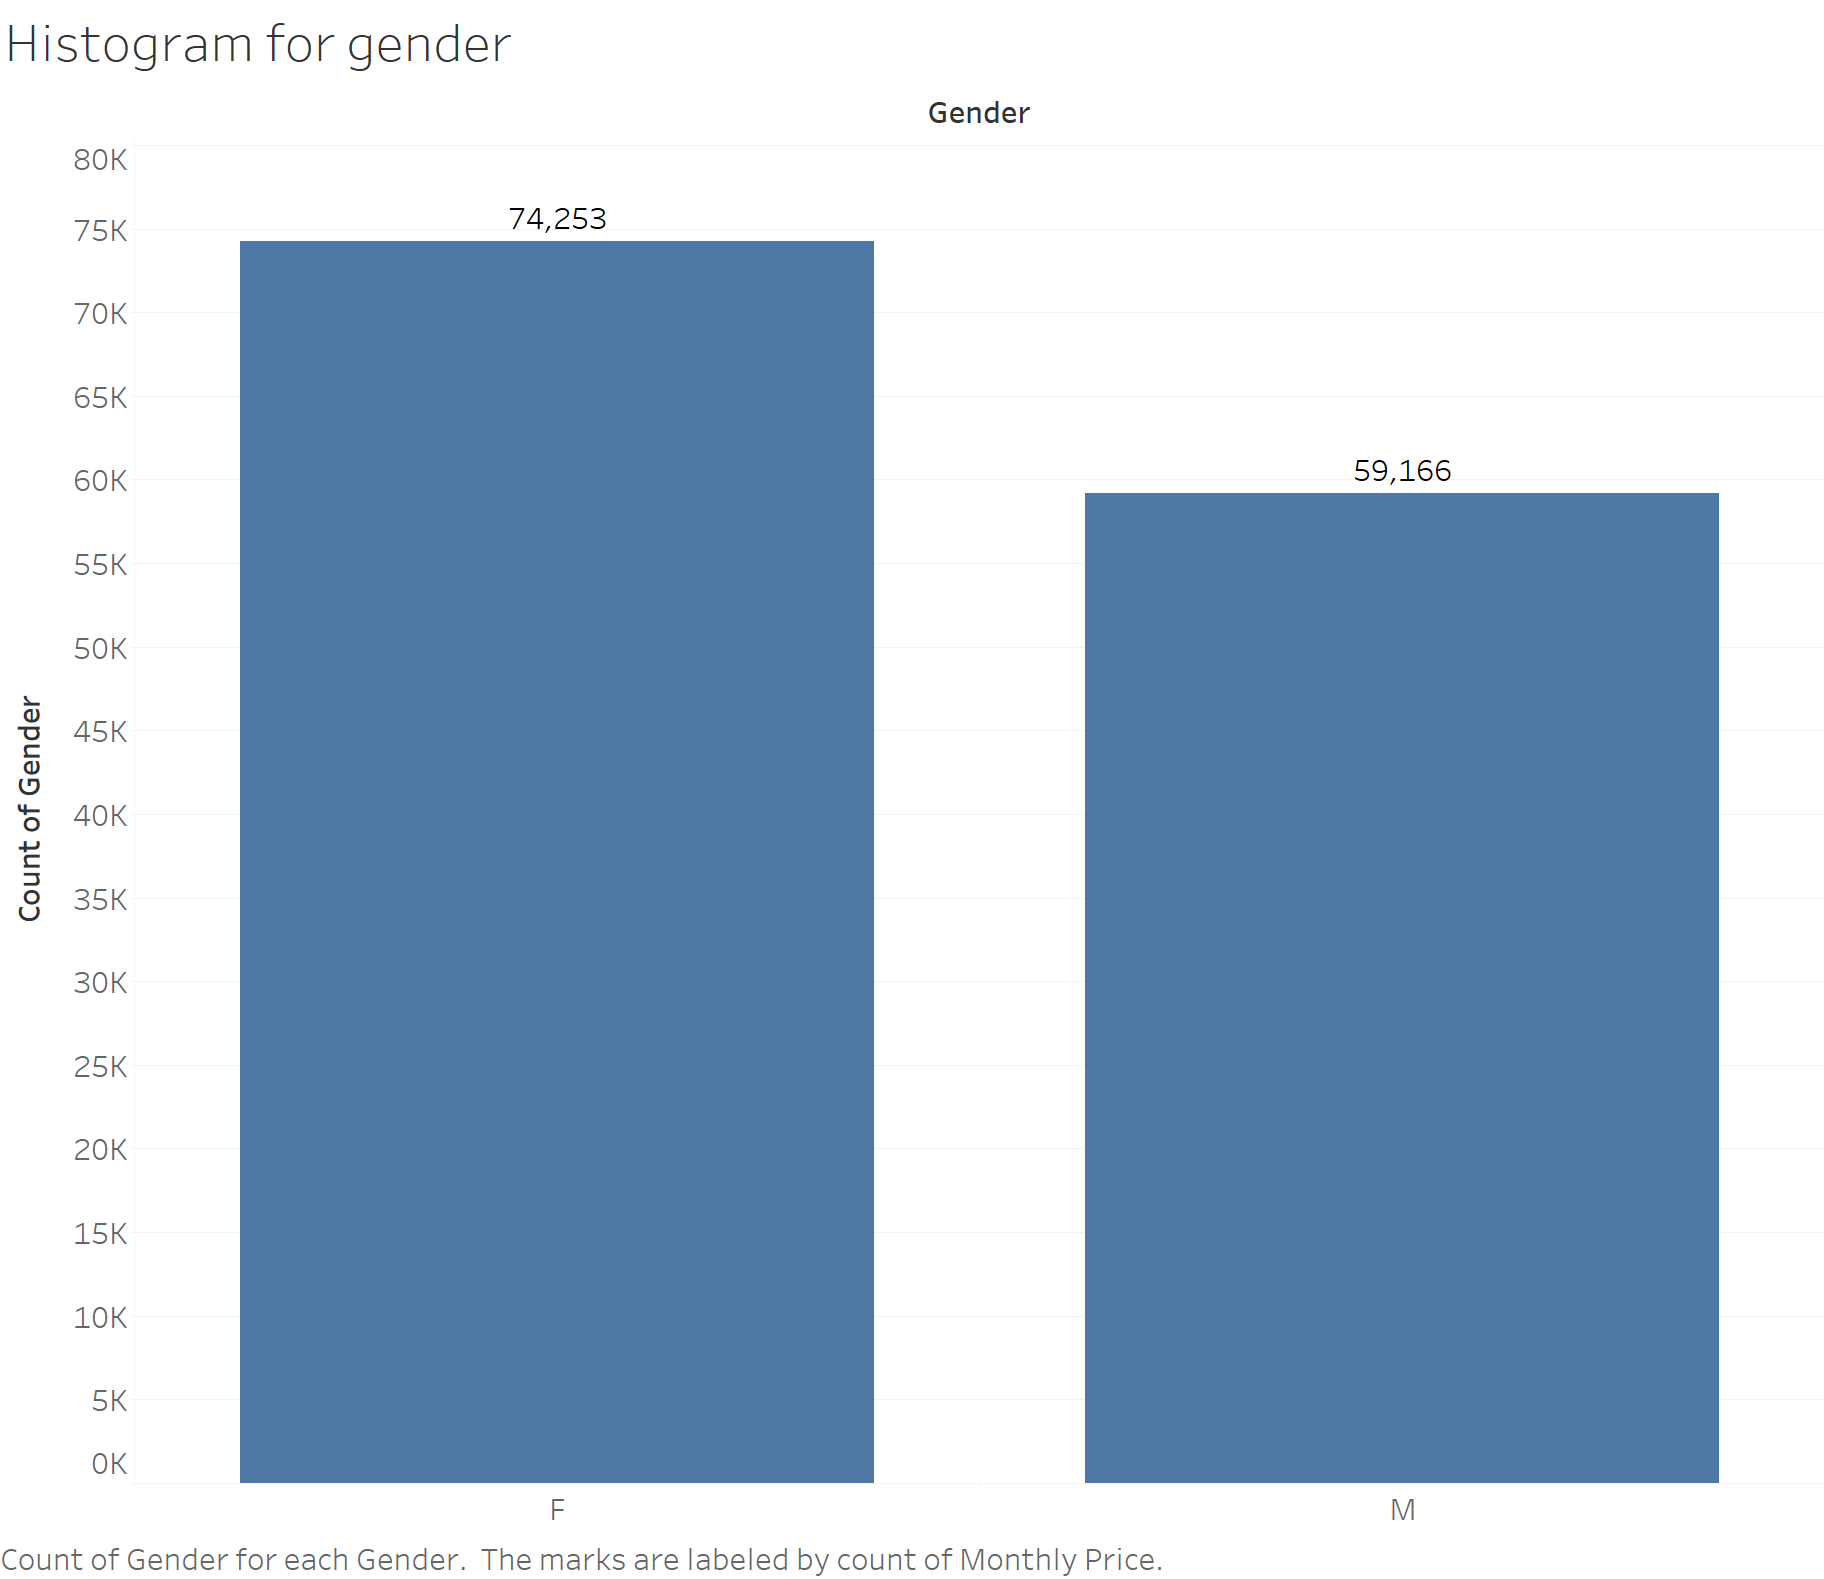
\includegraphics[width=0.8\columnwidth]{gender} 
\caption[Lostic Regression Confusion Matrix]{Gender Histogram} % The text in the square bracket is the caption for the list of figures while the text in the curly brackets is the figure caption
\label{fig:gallery} 
\end{figure}

\subsection{Sports}

\begin{figure}[H]
\centering 
\includegraphics[width=0.8\columnwidth]{Sport} 
\caption[Lostic Regression Confusion Matrix]{Gender Histogram} % The text in the square bracket is the caption for the list of figures while the text in the curly brackets is the figure caption
\label{fig:gallery} 
\end{figure}
 
 \subsection{Search Hits}
 
 \begin{figure}[H]
\centering 
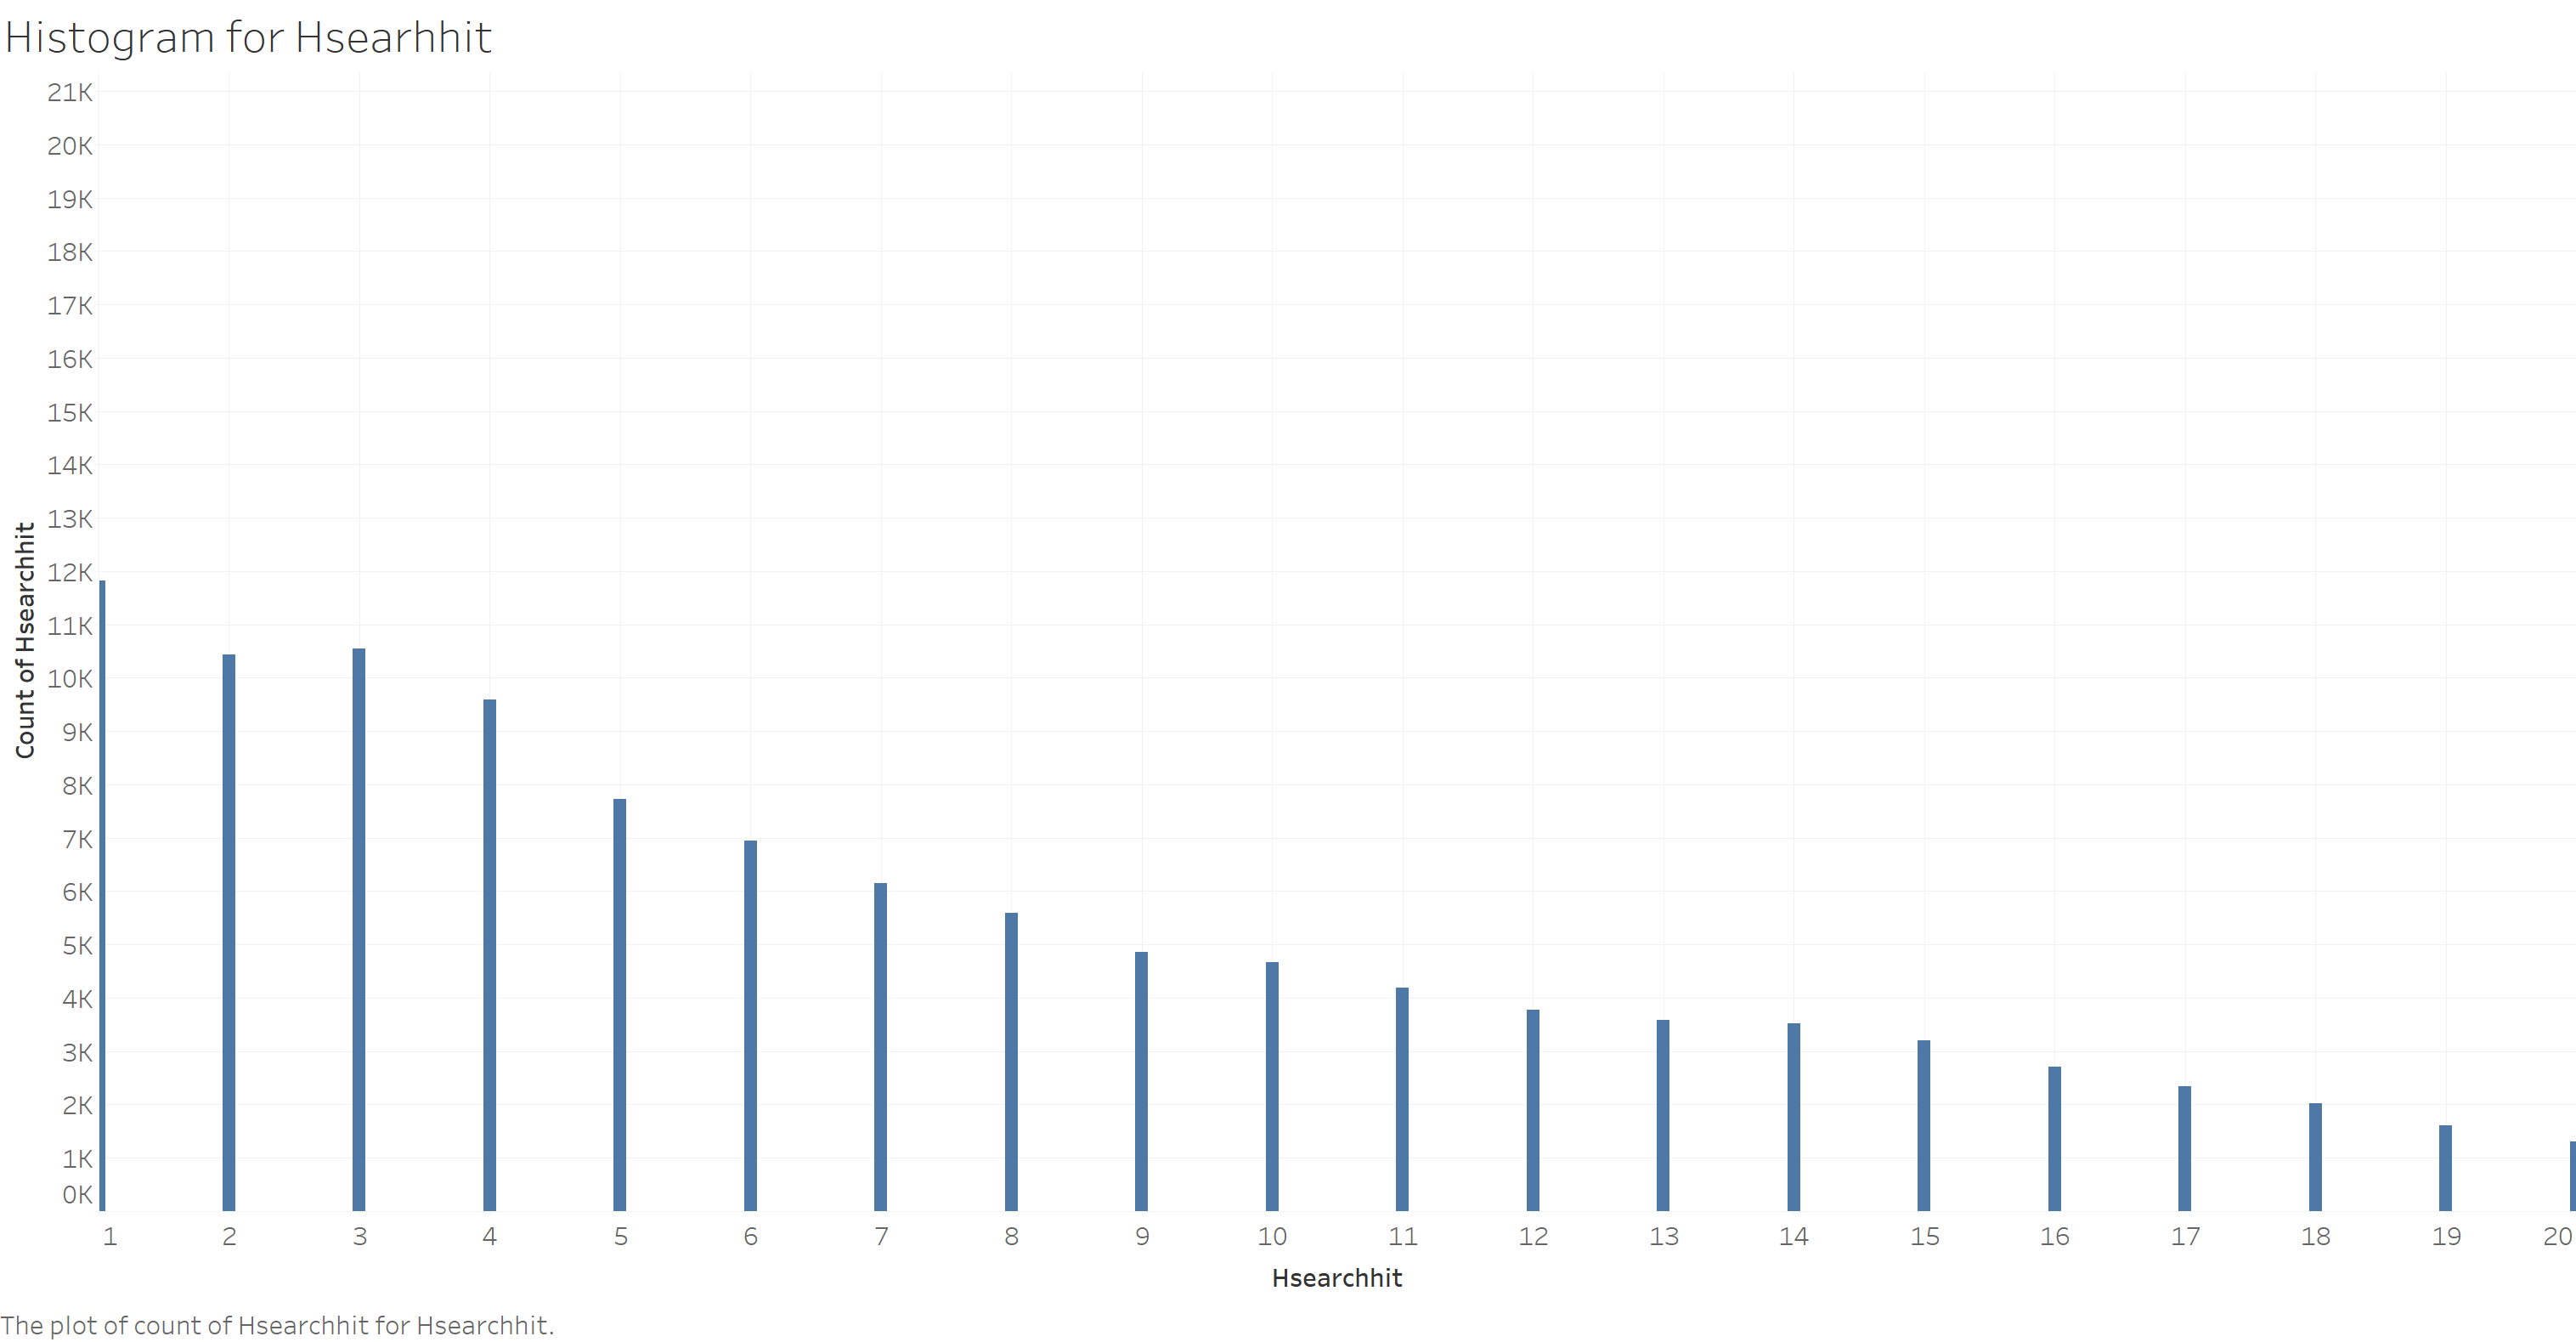
\includegraphics[width=0.8\columnwidth]{hsearchhit} 
\caption[Lostic Regression Confusion Matrix]{ hsearchhit Histogram} % The text in the square bracket is the caption for the list of figures while the text in the curly brackets is the figure caption
\label{fig:gallery} 
\end{figure}

\subsection{Duration}
 \begin{figure}[H]
\centering 
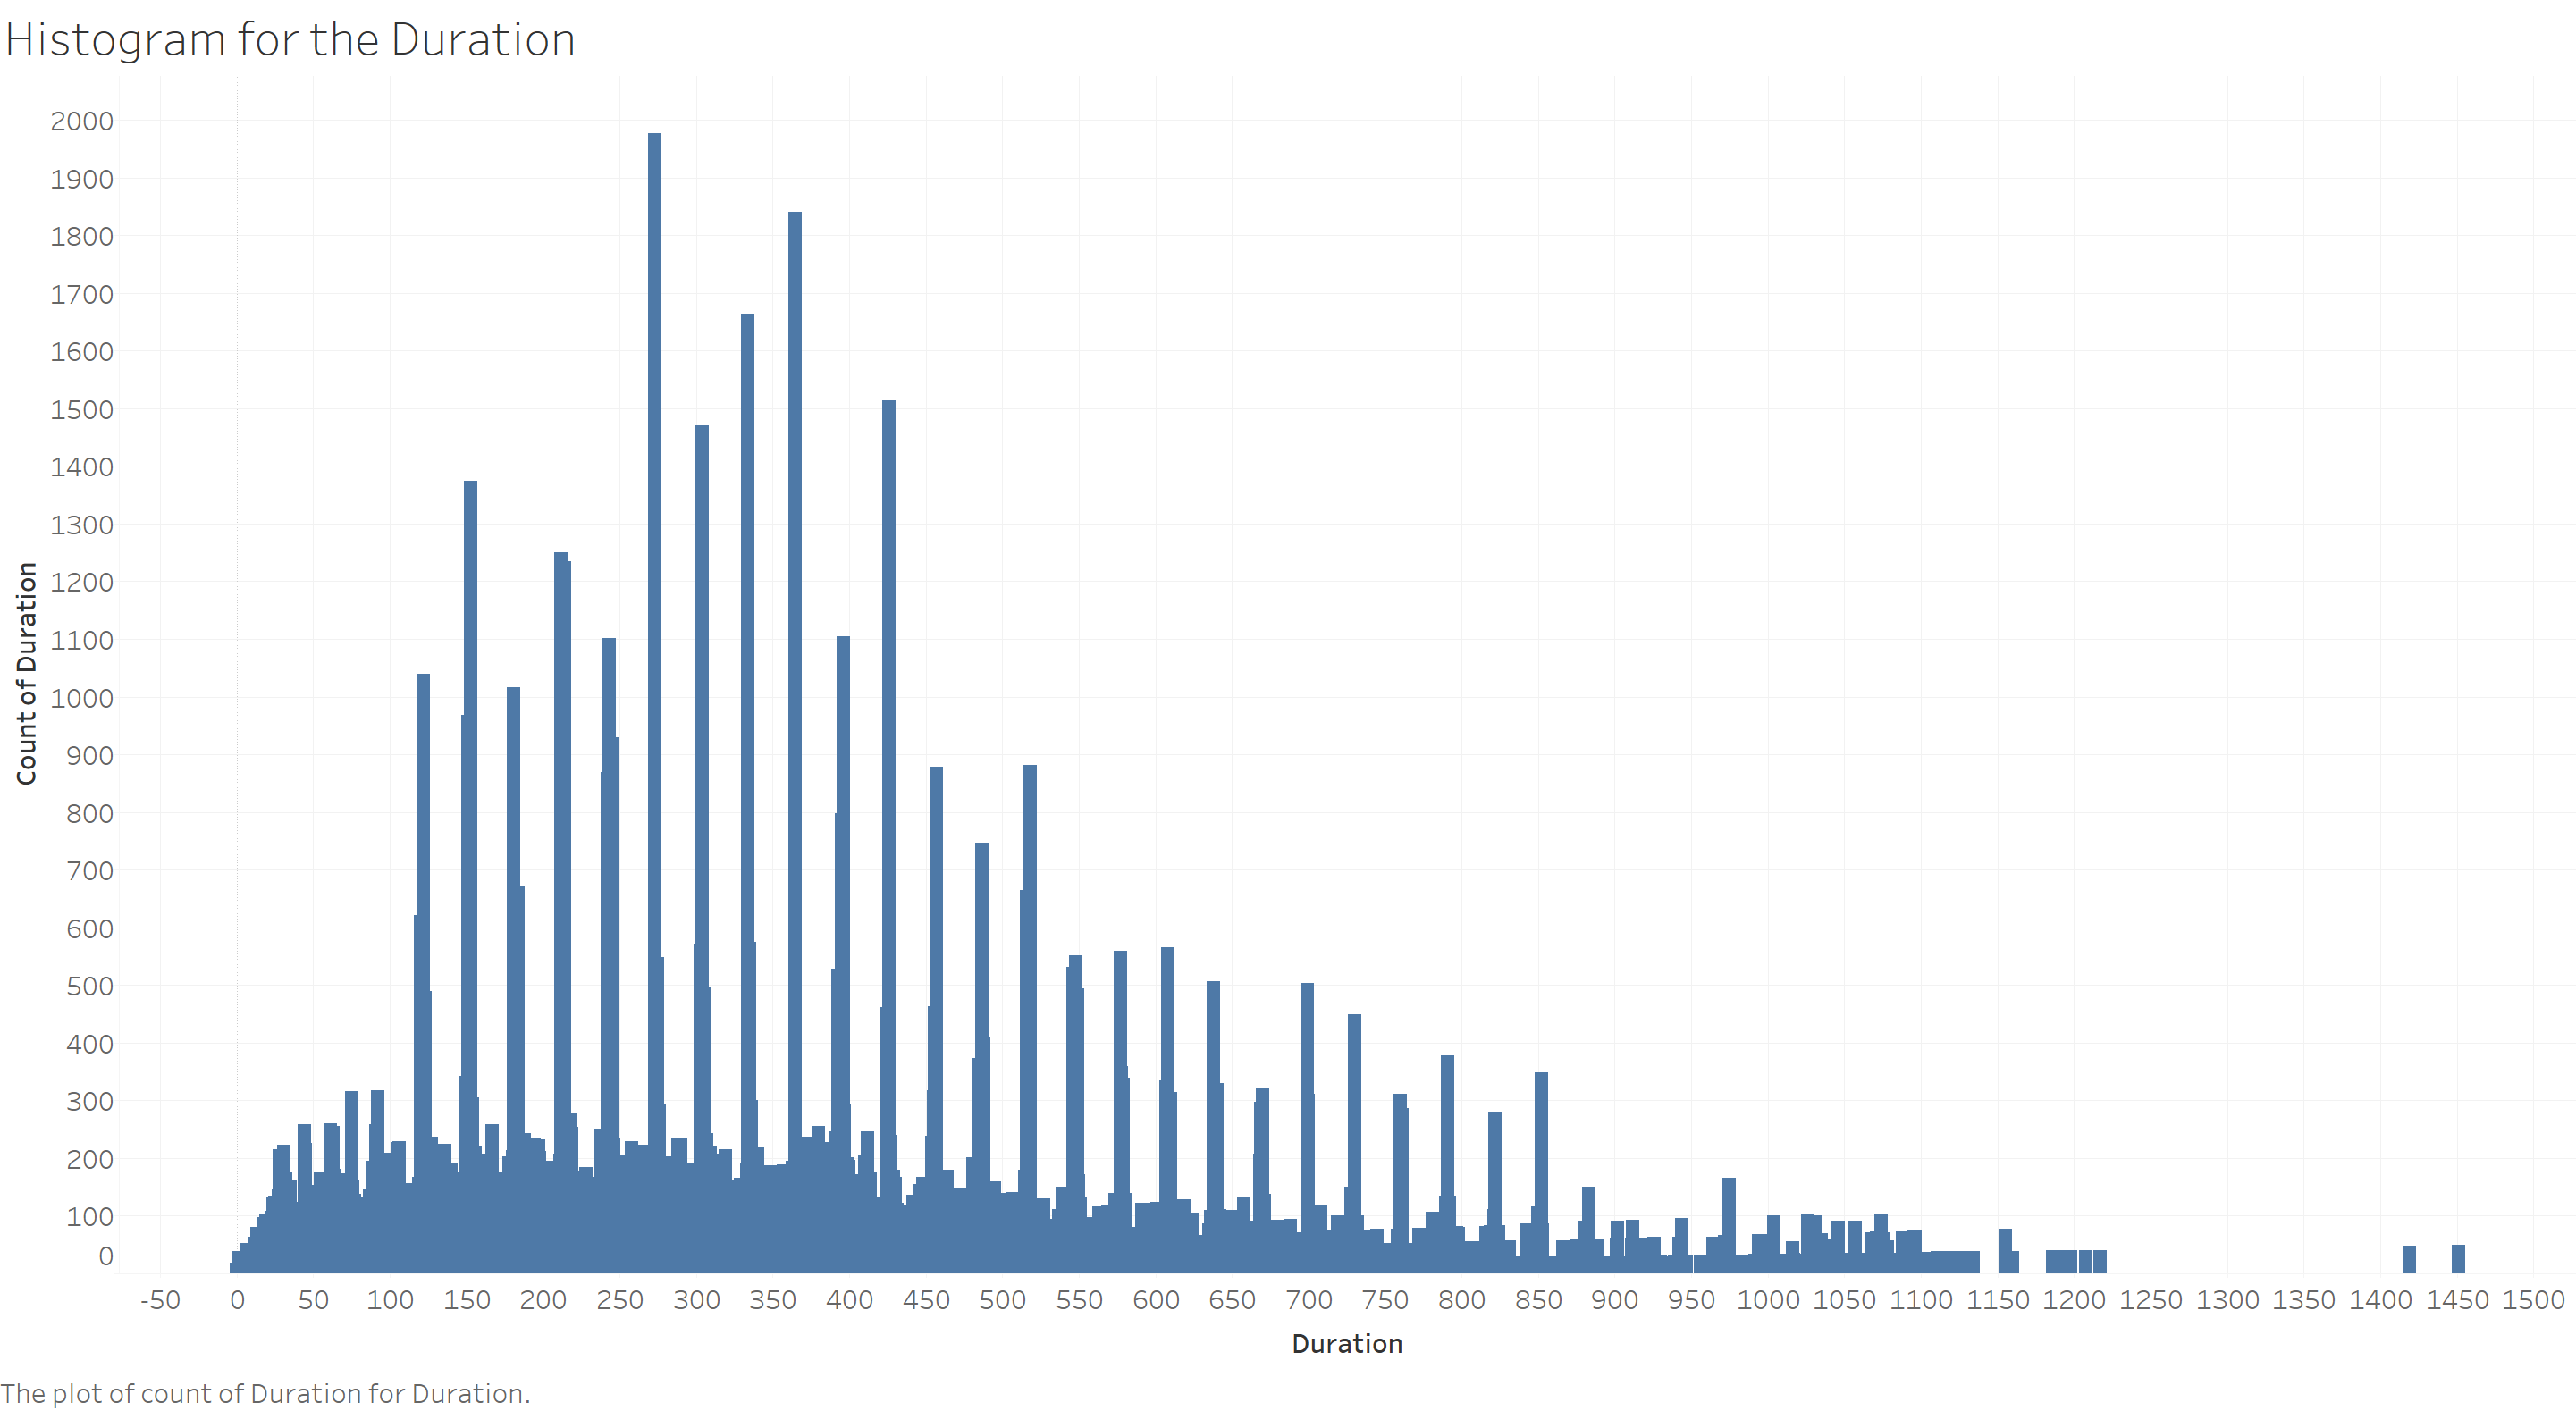
\includegraphics[width=0.8\columnwidth]{duration} 
\caption[Lostic Regression Confusion Matrix]{Duration Histogram} % The text in the square bracket is the caption for the list of figures while the text in the curly brackets is the figure caption
\label{fig:gallery} 
\end{figure}



%----------------------------------------------------------------------------------------
%	EVALUATION METHODS
%----------------------------------------------------------------------------------------

\section{Evaluation Metrics}

These are measures we used to determine how good our machine learning models were. We used the testing data to evaluate the model fitted using the training data. We shall briefly explain the measures we used and present the formula. Before then, we shall present two variables we shall use in the proceeding equations. 

\begin{itemize}
\item True Positive(TP) - These are the athletes who are predicted by the model to be most likely to churn and actually churned.
\item True Negative(TN) - These are the athletes who are predicted by the model to be most likely to be retained  and actually are retained.
\item False Positive(TP) - These are the athletes who are predicted by the model to be most likely to churn and actually are retained.
\item False Negative(TN) - These are the athletes who are predicted by the model to be most likely to be retained  and actually churned.

\end{itemize}

\subsection{Precision}
In the churn context, precision refers to how pure our predicted set is. Given a set of prediction of churners, how many of them are actually churners(True Positive (TP))?
\begin{align*}
  Precision = \frac{TP}{TP+FP}
\end{align*}

\subsection{Recall}
Given a set of churners, recall refers to the fraction of churners that the model correctly returns.
\begin{align*}
  Recall = \frac{TP}{TP+FN}
\end{align*}

\subsection{F1 Score}

This is the harmonic mean of precision and recall. 
\begin{align*}
  Recall = \frac{Precision * Recall}{Precision + Recall}
\end{align*}


%----------------------------------------------------------------------------------------
%	METHODS
%----------------------------------------------------------------------------------------

\section{One Month Churn Prediction Approaches}

We used March 2014 to predict churn in the next month. Predicting churn in the next month entailed setting the output variable (CaptainU\_Churn) of the training and testing datasets to the output variable of the next month.
\begin{table}[]
\centering
\caption{Dataset Attributes}
\label{my-label}
\begin{tabular}{@{}lllll@{}}
\toprule
Dataset  & Rows & columns & Churners & Non-Churners \\ \midrule
Full     & 4360 & 26      & 601      & 3759         \\
Training & 3488 & 26      & 484      & 3004         \\
Testing  & 872  & 26      & 117      & 755          \\ \bottomrule
\end{tabular}
\end{table}



%Reference to Figure~\vref{fig:gallery}. % The \vref command specifies the location of the reference


We implemented the following models in predicting churn:
\begin{enumerate}[noitemsep] % [noitemsep] removes whitespace between the items for a compact look
\item Logistic Regression 
\item Logistic Regression with (class\_weight = `balanced') - This mode uses the values of y(CaptainU\_CHURN) to automatically adjusts weights inversely proportional to class frequencies in the test data. Effectively, more attention was paid to churners as they make up the minority class.  You can read more about class\_weight \href{http://scikit-learn.org/stable/modules/generated/sklearn.linear_model.LogisticRegression.html}{here}
\item Gradient Boosting 
\item Random Forest Classifier 
\end{enumerate}

We then calculated the precision and recall values for churning. 


%------------------------------------------------

\subsection{Using a Specific Month's Transactions Data}

This is entailed tracking an athlete's monthly transactions and using that information to predict whether the athlete would churn in the next month. In our case for instance, we used March 2014's transaction data to predict if an athlete will churn in April 2014.

\subsubsection{Precision Recall Table} 

\begin{table}[H]
\centering
\caption{Precision Recall Values}
\label{my-label}
\begin{tabular}{@{}llll@{}}
\toprule
Model               & Precision & Recall & F1-Score \\ \midrule
Logistic Regression & 0.65      & 0.26   & 0.38     \\
Logistic Regression(with class\_weight = `balanced') & 0.43      & 0.56   & 0.49     \\
Random Forest       & 0.53      & 0.35   & 0.42     \\
Gradient Boosting   & 0.59      & 0.33   & 0.43     \\ \bottomrule
\end{tabular}
\end{table}

\subsubsection{\textbf{Confusion Matrix}: Logistic Regression}

\begin{figure}[H]
\centering 
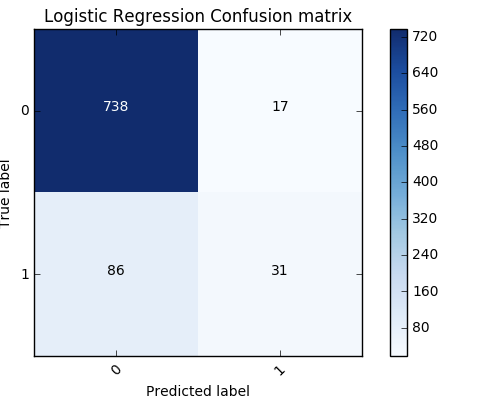
\includegraphics[width=0.8\columnwidth]{Logistic_One} 
\caption[Lostic Regression Confusion Matrix]{Lostic Regression Confusion Matrix} % The text in the square bracket is the caption for the list of figures while the text in the curly brackets is the figure caption
\label{fig:gallery} 
\end{figure}

The above confusion matrix illustrates the following: 

Given 117 athletes who are churners the model will:

\begin{itemize}
\item correctly predict 31 of the 117 athletes. 
\item incorrectly predict 17 athlete as having churned 
\item incorrectly predict 86 athletes as having been retained while in reality they are churners
\end{itemize}

\begin{figure}[H]
\centering 
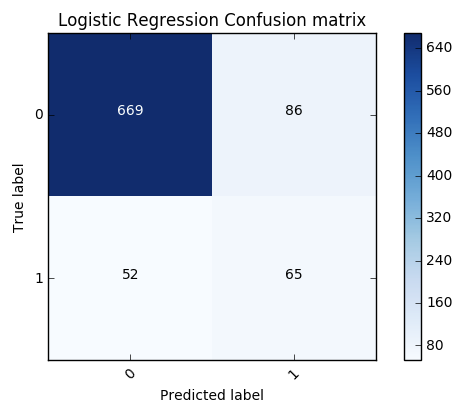
\includegraphics[width=0.8\columnwidth]{Logistic_Class} 
\caption[Lostic Regression Confusion Matrix]{Lostic Regression(class\_weight = `balanced') } % The text in the square bracket is the caption for the list of figures while the text in the curly brackets is the figure caption
\label{fig:gallery} 
\end{figure}

The above confusion matrix illustrates the following: 
Given 117 athletes who are churners the model will:

\begin{itemize}
\item correctly predict 65 of the 117 athletes. 
\item incorrectly predict 86 athlete as having churned 
\item incorrectly predict 52 athletes as having been retained while in reality they are churners
\end{itemize}
\subsubsection{\textbf{Confusion Matrix}: Random Forest}


\begin{figure}[H]
\centering 
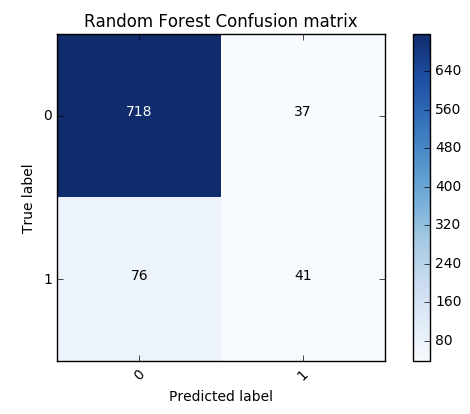
\includegraphics[width=0.8\columnwidth]{Random_F_One} 
\caption[Lostic Regression Confusion Matrix]{Random Forest Confusion Matrix} % The text in the square bracket is the caption for the list of figures while the text in the curly brackets is the figure caption
\label{fig:gallery} 
\end{figure}
The above confusion matrix illustrates the following: 

Given 117 athletes who are churners the model will:

\begin{itemize}
\item correctly predict 41 of the 117 athletes. 
\item incorrectly predict 37 athlete as having churned 
\item incorrectly predict 76 athletes as having been retained while in reality they are churners
\end{itemize}

\subsubsection{\textbf{Confusion Matrix}: Gradient Boosting}

\begin{figure}[H]
\centering 
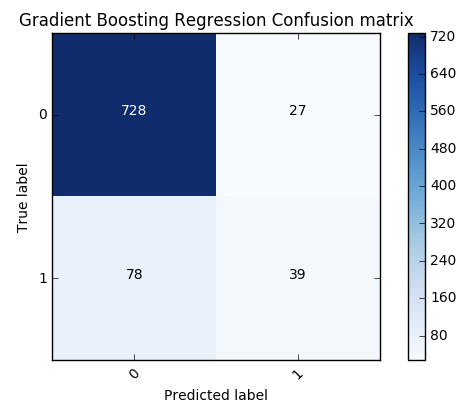
\includegraphics[width=0.8\columnwidth]{Gradient_F_One} 
\caption[Lostic Regression Confusion Matrix]{Gradient Boosting Confusion Matrix} % The text in the square bracket is the caption for the list of figures while the text in the curly brackets is the figure caption
\label{fig:gallery} 
\end{figure}

The above confusion matrix illustrates the following: 

Given 117 athletes who are churners the model will:

\begin{itemize}
\item correctly predict 39 of the 117 athletes. 
\item incorrectly predict 27 athlete as having churned 
\item incorrectly predict 78 athletes as having been retained while in reality they are churners
\end{itemize}


%------------------------------------------------

\subsection{Using Aggregate Transactions Data}

This is entailed tracking an athlete's aggregate transactions data up to a certain month and using that information to predict whether the athlete would churn in the next month. In our case, we used the cumulative sum of each feature up to March 2014 to predict churn in April 2014.

\subsubsection{Precision Recall Table} 

\begin{table}[H]
\centering
\caption{Precision Recall Values}
\label{my-label}
\begin{tabular}{@{}llll@{}}
\toprule
Model               & Precision & Recall & F1-Score \\ \midrule
Logistic Regression & 0.00      & 0.00   & 0.00     \\
Logistic Regression(with class\_weight = `balanced') & 0.18      & 0.61   & 0.28     \\
Random Forest       & 0.00      & 0.00   & 0.00     \\
Gradient Boosting   & 0.50      & 0.02   & 0.03     \\ \bottomrule
\end{tabular}
\end{table}

\subsubsection{\textbf{Confusion Matrix}: Logistic Regression}

\begin{figure}[H]
\centering 
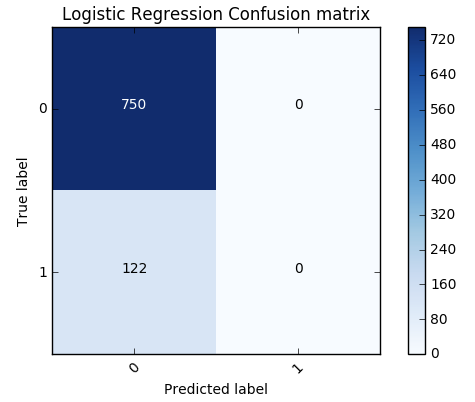
\includegraphics[width=0.8\columnwidth]{Logistic_Freq} 
\caption[Lostic Regression Confusion Matrix]{Lostic Regression Confusion Matrix} % The text in the square bracket is the caption for the list of figures while the text in the curly brackets is the figure caption
\label{fig:gallery} 
\end{figure}

The above confusion matrix illustrates the following: 

Given 117 athletes who are churners the model will:

\begin{itemize}
\item correctly predict none of the 117 athletes. 
\item incorrectly predict 0 athletes as having churned 
\item incorrectly predict 122 athletes as having been retained while in reality 117 of them are churners
\end{itemize}

\begin{figure}[H]
\centering 
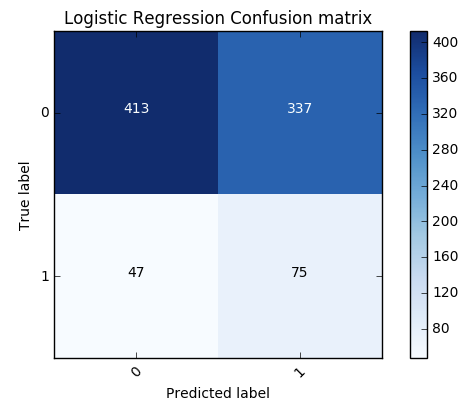
\includegraphics[width=0.8\columnwidth]{Logistic_Freq_CW} 
\caption[Lostic Regression Confusion Matrix]{Lostic Regression with class\_weight='balanced'} % The text in the square bracket is the caption for the list of figures while the text in the curly brackets is the figure caption
\label{fig:gallery} 
\end{figure}

The above confusion matrix illustrates the following: 

Given 117 athletes who are churners the model will:

\begin{itemize}
\item correctly predict 75 of the 117 athletes. 
\item incorrectly predict 337 athletes as having churned 
\item incorrectly predict 47 athletes as having been retained while in reality 117 of them are churners
\end{itemize}

\subsubsection{\textbf{Confusion Matrix}: Random Forest}

\begin{figure}[H]
\centering 
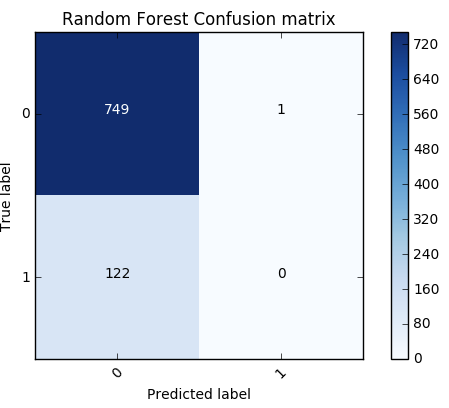
\includegraphics[width=0.8\columnwidth]{Rand_Freq} 
\caption[Lostic Regression Confusion Matrix]{Random Forest Confusion Matrix. } % The text in the square bracket is the caption for the list of figures while the text in the curly brackets is the figure caption
\label{fig:gallery} 
\end{figure}

The above confusion matrix illustrates the following: 

Given 117 athletes who are churners the model will:

\begin{itemize}
\item correctly predict none of the 117 athletes. 
\item incorrectly predict 1 athlete as having churned 
\item incorrectly predict 122 athletes as having been retained while in reality 117 of them are churners
\end{itemize}

\subsubsection{\textbf{Confusion Matrix}: Gradient Boosting}

\begin{figure}[H]
\centering 
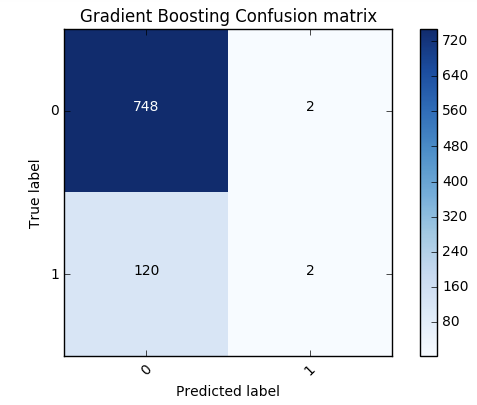
\includegraphics[width=0.8\columnwidth]{Gradient_Freq} 
\caption[Lostic Regression Confusion Matrix]{Gradient Boosting Confusion Matrix} % The text in the square bracket is the caption for the list of figures while the text in the curly brackets is the figure caption
\label{fig:gallery} 
\end{figure}

The above confusion matrix illustrates the following: 

Given 117 athletes who are churners the model will:

\begin{itemize}
\item correctly predict 2 of the 117 athletes. 
\item incorrectly predict 2 athletes as having churned 
\item incorrectly predict 120 athletes as having been retained while in reality 115 of them are churners
\end{itemize}

\pagebreak
%------------------------------------------------

\subsection{Using Monthly Difference in Transactions Data}

This is entailed tracking an athlete's change in transactions data from one month to the next and using that information to predict whether the athlete would churn in the next month. For instance, we would track the change in the number of hits between February 2014 and March 2014 and Creating a Hits\_diff column. For creating our testing and training data, we tracked the difference in transactions(interactions) between February 2014 and March 2014 to predict churn in April 2014.

\subsubsection{Precision Recall Table} 

\begin{table}[H]
\centering
\caption{Precision Recall Values}
\label{my-label}
\begin{tabular}{@{}llll@{}}
\toprule
Model               & Precision & Recall & F1-Score \\ \midrule
Logistic Regression & 0.00      & 0.00   & 0.00     \\
Logistic Regression(with class\_weight = `balanced') & 0.07      & 0.55   & 0.13     \\
Random Forest       & 0.00      & 0.00   & 0.00     \\
Gradient Boosting   & 0.10      & 0.02   & 0.03     \\ \bottomrule
\end{tabular}
\end{table}

\subsubsection{\textbf{Confusion Matrix}: Logistic Regression}

\begin{figure}[H]
\centering 
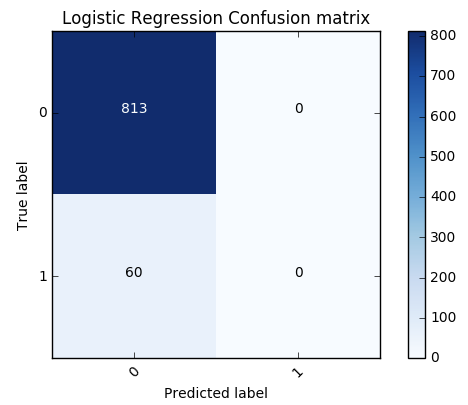
\includegraphics[width=0.8\columnwidth]{Logic_diff} 
\caption[Lostic Regression Confusion Matrix]{Lostic Regression Confusion Matrix} % The text in the square bracket is the caption for the list of figures while the text in the curly brackets is the figure caption
\label{fig:gallery} 
\end{figure}

The above confusion matrix illustrates the following: 

Given 117 athletes who are churners the model will:

\begin{itemize}
\item correctly predict none of the 117 athletes. 
\item incorrectly predict 0 athlete as having churned 
\item incorrectly predict 60 athletes as having been retained 
\end{itemize}

\begin{figure}[H]
\centering 
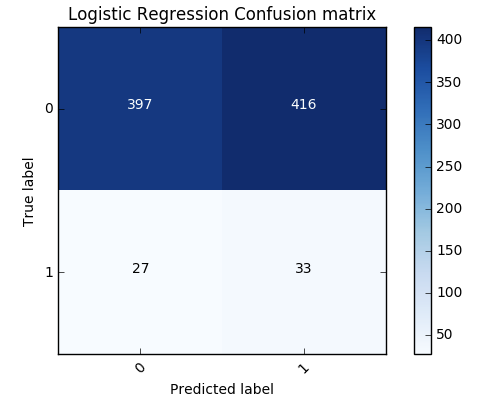
\includegraphics[width=0.8\columnwidth]{Logic_diff_CW} 
\caption[Lostic Regression Confusion Matrix]{Lostic Regression with class\_weight='balanced'} % The text in the square bracket is the caption for the list of figures while the text in the curly brackets is the figure caption
\label{fig:gallery} 
\end{figure}

The above confusion matrix illustrates the following: 

Given 117 athletes who are churners the model will:

\begin{itemize}
\item correctly predict 33 of the 117 athletes. 
\item incorrectly predict 416 athlete as having churned 
\end{itemize}

\subsubsection{\textbf{Confusion Matrix}: Random Forest}

\begin{figure}[H]
\centering 
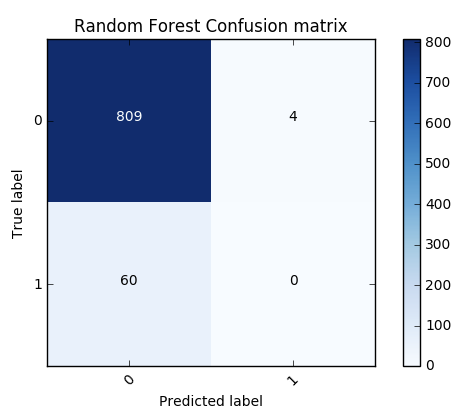
\includegraphics[width=0.8\columnwidth]{Rand_diff} 
\caption[Lostic Regression Confusion Matrix]{Random Forest Confusion Matrix. We Suspect Overfitting here} % The text in the square bracket is the caption for the list of figures while the text in the curly brackets is the figure caption
\label{fig:gallery} 
\end{figure}

\subsubsection{\textbf{Confusion Matrix}: Gradient Boosting}

\begin{figure}[H]
\centering 
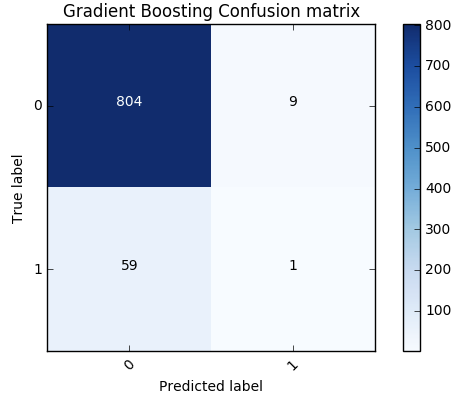
\includegraphics[width=0.8\columnwidth]{GB_diff} 
\caption[Lostic Regression Confusion Matrix]{Gradient Boosting Confusion Matrix} % The text in the square bracket is the caption for the list of figures while the text in the curly brackets is the figure caption
\label{fig:gallery} 
\end{figure}

The above confusion matrix illustrates the following: 

Given 10 athletes who are predicted to have churned, only one actually churns.

\section{Life-time Churn Prediction}

The models we built here were geared towards answering the question: Will athlete A churn at some point in their high school career before:

\begin{itemize}
\item Making a team
\item His/her spring semester of his/her senior year
\end{itemize}

\subsection{Dataset Attributes}
To create the dataset for this model, we aggregated each feature and set the churn value(CaptainU\_CHURN) to the value of the last month the athlete was on the system or the value on December 1st 2014. This is because all athletes in the system had churned in January 2015(Spring semester of their senior year). 

\begin{table}[H]
\centering
\caption{My caption}
\label{my-label}
\begin{tabular}{@{}lllll@{}}
\toprule
Dataset  & Rows  & columns & Churners & Non-Churners \\ \midrule
Full     & 16117 & 26      & 6043     & 10074        \\
Training & 12893 & 26      & 4832     & 8061         \\
Testing  & 3224  & 26      & 1211     & 2013         \\ \bottomrule
\end{tabular}
\end{table}

\subsection{Churn in both males and Females}
\subsubsection{Precision Recall Table}

\begin{table}[H]
\centering
\caption{Precision Recall Values}
\label{my-label}
\begin{tabular}{@{}llll@{}}
\toprule
Model               & Precision & Recall & F1-Score \\ \midrule
Logistic Regression & 0.75      & 0.68   & 0.71     \\
Logistic Regression(with class\_weight = `balanced') & 0.65      & 0.82   & 0.73     \\
Random Forest       & 0.79      & 0.72   & 0.75     \\
Gradient Boosting   & 0.77      & 0.75   & 0.76     \\ 
Support Vector Machine   & 0.75      & 0.67   & 0.71     \\  \bottomrule
\end{tabular}
\end{table}

\subsubsection{Confusion Matrix: Logistic Regression}

\begin{figure}[H]
\centering 
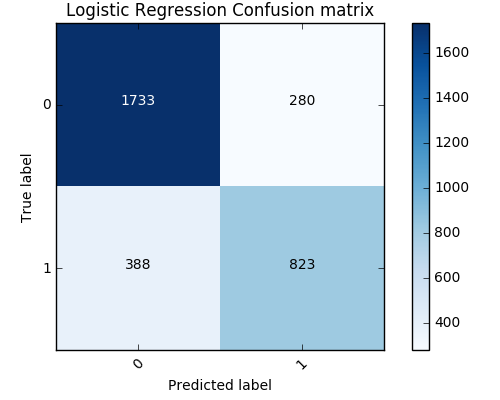
\includegraphics[width=0.8\columnwidth]{Logic_Life} 
\caption[Lostic Regression Confusion Matrix]{Lostic Regression Confusion Matrix} % The text in the square bracket is the caption for the list of figures while the text in the curly brackets is the figure caption
\label{fig:gallery} 
\end{figure}

The above confusion matrix illustrates the following: 

Given 1211 athletes who are churners the model will:

\begin{itemize}
\item correctly predict 823 of the 1211 athletes. 
\item incorrectly predict 280 athlete as having churned 
\item incorrectly predict 388 athletes as having been retained while in reality they churned
\end{itemize}

\subsubsection{Confusion Matrix: Logistic Regression with balanced class weight}

\begin{figure}[H]
\centering 
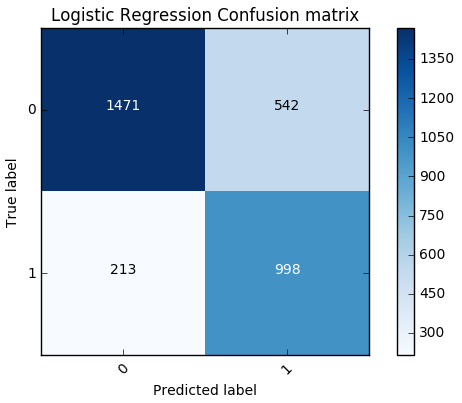
\includegraphics[width=0.8\columnwidth]{Logic_Life_CW} 
\caption[Lostic Regression Confusion Matrix]{Lostic Regression Confusion Matrix} % The text in the square bracket is the caption for the list of figures while the text in the curly brackets is the figure caption
\label{fig:gallery} 
\end{figure}

The above confusion matrix illustrates the following: 

Given 1211 athletes who are churners the model will:

\begin{itemize}
\item correctly predict 998 of the 1211 athletes. 
\item incorrectly predict 542 athlete as having churned 
\item incorrectly predict 213 athletes as having been retained while in reality they churned
\end{itemize}

Effectively, this means that 2 of the 3 athletes who are predicted to churn at some point in the future are actually churners.

\subsubsection{Confusion Matrix: Random Forest}

\begin{figure}[H]
\centering 
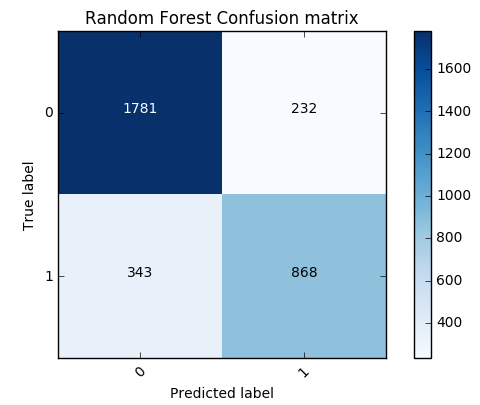
\includegraphics[width=0.8\columnwidth]{RF_Life} 
\caption[Lostic Regression Confusion Matrix]{Random Forest Confusion Matrix} % The text in the square bracket is the caption for the list of figures while the text in the curly brackets is the figure caption
\label{fig:gallery} 
\end{figure}

The above confusion matrix illustrates the following: 

Given 1211 athletes who are churners the model will:

\begin{itemize}
\item correctly predict 868 of the 1211 athletes. 
\item incorrectly predict 232 athlete as having churned 
\item incorrectly predict 343 athletes as having been retained while in reality they churned
\end{itemize}

Effectively, this means that about 8 of the 10 athletes who are predicted to churn at some point in the future are actual churners.

\subsubsection{Confusion Matrix: Gradient Boosting}

\begin{figure}[H]
\centering 
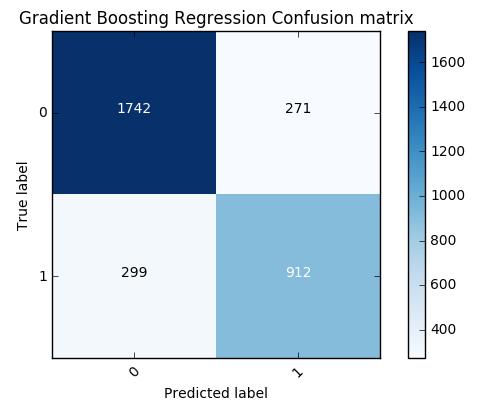
\includegraphics[width=0.8\columnwidth]{GB_Life} 
\caption[Lostic Regression Confusion Matrix]{Random Forest Confusion Matrix} % The text in the square bracket is the caption for the list of figures while the text in the curly brackets is the figure caption
\label{fig:gallery} 
\end{figure}

The above confusion matrix illustrates the following: 

Given 1211 athletes who are churners the model will:

\begin{itemize}
\item correctly predict 868 of the 1211 athletes. 
\item incorrectly predict 232 athlete as having churned 
\item incorrectly predict 343 athletes as having been retained while in reality they churned
\end{itemize}

Effectively, this means that about 8 of the 10 athletes who are predicted to churn at some point in the future are actual churners.

\subsection{Churn in Males}

We went ahead and isolated males and tried to understand what factors lead to churn in males. 

\subsubsection{Dataset Attributes}

\begin{table}[H]
\centering
\caption{Dataset attributes}
\label{my-label}
\begin{tabular}{@{}lllll@{}}
\toprule
Dataset  & Rows  & columns & Churners & Non-Churners \\ \midrule
Full     & 7342 & 26      & 2334     & 5008        \\
Training & 5873 & 26      & 1869     & 4004         \\
Testing  & 1469  & 26      & 465     & 1004         \\ \bottomrule
\end{tabular}
\end{table}

\subsubsection{Precision Recall Table}

\begin{table}[H]
\centering
\caption{Precision Recall Values}
\label{my-label}
\begin{tabular}{@{}llll@{}}
\toprule
Model               & Precision & Recall & F1-Score \\ \midrule
Logistic Regression & 0.72      & 0.63   & 0.67     \\
Gradient Boosting   & 0.77      & 0.72   & 0.74     \\  \bottomrule
\end{tabular}
\end{table}

\subsubsection{Important features}
We visualised the most important features that lead to either churn or retention. The features in blue lead to churn while the the features in read drive retention.  This is because positive coefficients increase the log-odds of the response (and thus increase the probability), and negative coefficients decrease the log-odds of the response (and thus decrease the probability).The values on the y-axis represent the weight values of each features based on the logistic regression equation:

\begin{align*}
  F(x) = \frac{1}{1+e^{-\beta_i}}
\end{align*}

\begin{figure}[H]
\centering 
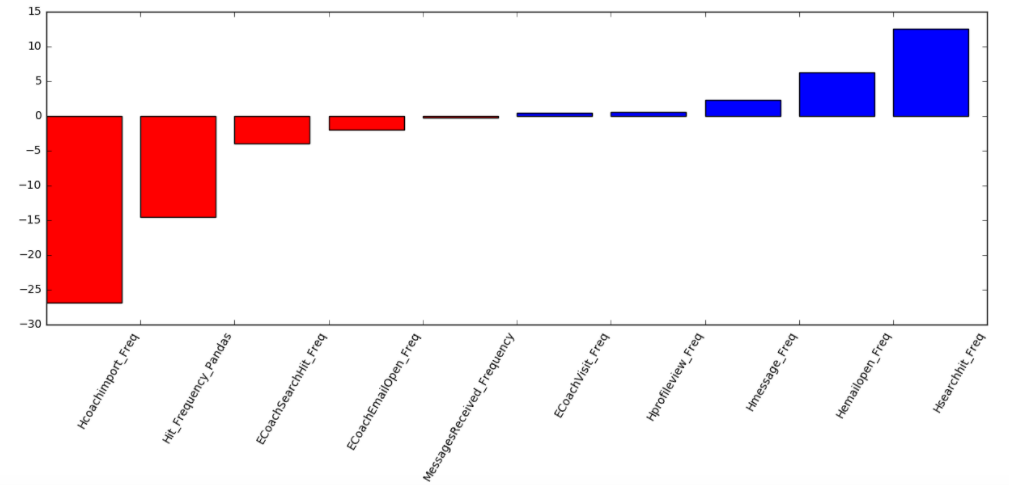
\includegraphics[width=0.8\columnwidth]{Logic_M} 
\caption[Lostic Regression Confusion Matrix]{Important Features Affecting Churnin Males} % The text in the square bracket is the caption for the list of figures while the text in the curly brackets is the figure caption
\label{fig:gallery} 
\end{figure}
In figure above, we can postulate that the more a coach imports an athlete's information and the more an athlete gets profile hits, the more he is likely to stay.

\subsection{Churn in Females}

\subsubsection{Dataset Attributes}
\begin{table}[H]
\centering
\caption{My caption}
\label{my-label}
\begin{tabular}{@{}lllll@{}}
\toprule
Dataset  & Rows  & columns & Churners & Non-Churners \\ \midrule
Full     & 8775 & 26      & 3759     & 5066        \\
Training & 7020 & 26      & 2994     & 4076         \\
Testing  & 1755  & 26      & 765        & 990         \\ \bottomrule
\end{tabular}
\end{table}

\subsubsection{Precision Recall Table}

\begin{table}[H]
\centering
\caption{Precision Recall Values}
\label{my-label}
\begin{tabular}{@{}llll@{}}
\toprule
Model               & Precision & Recall & F1-Score \\ \midrule
Logistic Regression & 0.72      & 0.75   & 0.74     \\
Gradient Boosting   & 0.76      & 0.81   & 0.79     \\  \bottomrule
\end{tabular}
\end{table}

\subsubsection{Important features}
\begin{figure}[H]
\centering 
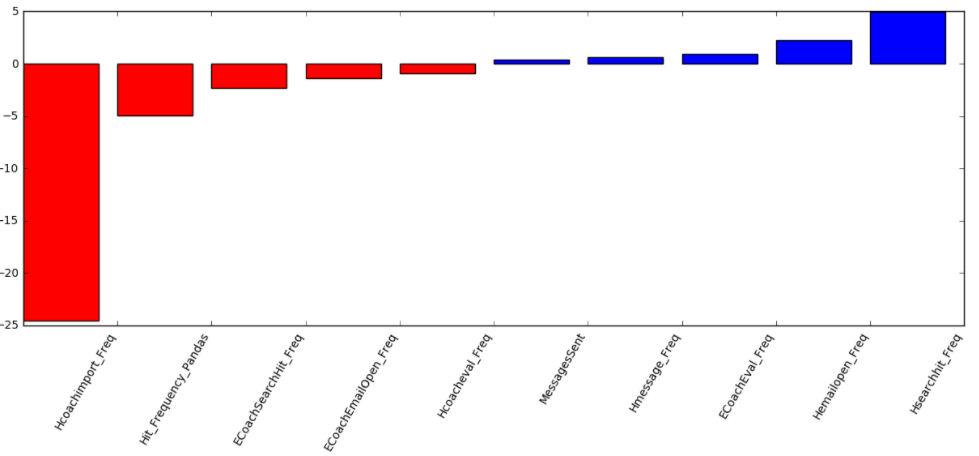
\includegraphics[width=0.8\columnwidth]{Logic_F} 
\caption[Lostic Regression Confusion Matrix]{Important Features Affecting Churn in Females} % The text in the square bracket is the caption for the list of figures while the text in the curly brackets is the figure caption
\label{fig:gallery} 
\end{figure}


%----------------------------------------------------------------------------------------
%	RESULTS AND DISCUSSION
%----------------------------------------------------------------------------------------
\newpage

\section{Results and Discussion}

These preliminary results for predicting monthly and life time churn. With there results, we can infer the following: 
\begin{itemize}
\item Predicting life time churn has gives better results than predicting one month churn. This is mostly due to the fact that the dataset is larger and the the split of churn and non churners is about 2:1.
\item Logistic regression is more consistent in providing credible results compared to random forest and gradient boosting

\end{itemize}

\newpage
\section{Future Work}

With every data science project, good results lie in data engineering. Our results mainly focused on the already assembled MSG\_RFM table, going forward, we would recommend making use of the other tables in the database. 


%Reference to Table~\vref{tab:label}. % The \vref command specifies the location of the reference


%----------------------------------------------------------------------------------------
%	BIBLIOGRAPHY
%----------------------------------------------------------------------------------------

\renewcommand{\refname}{\spacedlowsmallcaps{References}} % For modifying the bibliography heading

\bibliographystyle{unsrt}

\bibliography{sample.bib} % The file containing the bibliography

%----------------------------------------------------------------------------------------

\end{document}